The detectors are represented as game objects and children of the \texttt{Detectors} game object under each hand game object. 
Each of these detector objects have the naming convention <gesture name> + "Detector" + <optional specifier> + "\_" + <handedness: Left or Right>, 
e.g.~\texttt{PinchDetectorStrict\_Left} and \texttt{FistDetector\_Right}. A certain detector of one hand is usual identical to the equivalent detector for the 
other hand with a few exception. These differences between hands are usually minor and will be mentioned when applicable. The detectors used in this implementation
utilizes a combination of several Leap Motion provided detectors, as these both cover the functional needs and are considered best practice. 
The Leap Motion provided detectors can as such be regarded as "base detectors", while the detectors that represents gestures in this implementation
can be regarded as "composite detectors". To differentiate between these two categories, the base detectors will be written in \textit{italic} or plain text, while
the composite detectors and game objects will be written in \texttt{monospace}.
The Leap Motion provided detectors utilized in the implementation is \textit{DetectorLogicGate}, \textit{PinchDetector}, \textit{ExtendedFingerDetector}, 
\textit{PalmDirectionDetector} and \textit{FingerDirectionDetector}.

The Leap motion base detectors provides some important parameters that can be set on a per detector instance basis, which often relates to thresholds values (e.g.~on/off values) and discrete
values (e.g~extended or not extended). Finding the optimal values for a certain gesture can often be the subject of a lot of adjustment and tweaking, as vision-based gesture recognition
technology often or always will be someone unprecice compared to e.g.~mouse and keyboard. The challenge is thus to find values that give a high amout of true positives (e.g.~the user attemps a gesture
and the gesture was recognized) and a low amount of false positives (e.g.~the user did not attempt a gesture and a gesture was recognized). 
During the implementation phase these values were adjusted several times in pursuit of the optimal values, and during the evaluation phase this was a much discussed topic were users often 
has their own "gesture sensitivity preferences" (this will be review in the next chapter). 

As was mentioned in the design, giving the user visual feedback when a gesture is recognized (i.e a detector is active) is probably a good idea.
In this implementation this is performed by changing the material of the hand models. The materials for each hand is listed in the handMaterials variable in the
\texttt{GestureHand} class, and follows the same order (or indecies) as the HandState enums specify (see~\vref{tab:handstates}). 
Changing these materials is thus easy to do in Unity, but as default the following color-categories are used:
\begin{itemize}
\item Plain gold   - Used for gestures that perform rotations (only the pinch gesture).
\item Black 	   - Used for gestures that perform movement. This includes the Palm-down gesture (either y-axis movement or xyz-axes movement), 
			  		 Palm-side gesutre (x-axis movement) and the fist gesture (z-axis movement).
\item Glowing teal - Used for gestures that perform annotation interaction, i.e either places or edits annotations.
					 This includes the single point-gesture and the double point-gesture.
\item White 	   - Used when no gesture is performed (but gestures are still enabled).
\item Transparent  - Used when gestures are disabled.					
\end{itemize}

First the gesture implementations will be reviewed. 


\subsection{The PinchDetectorStrict and PinchDetectorSlack}
\begin{figure}%[h!] %[H]
	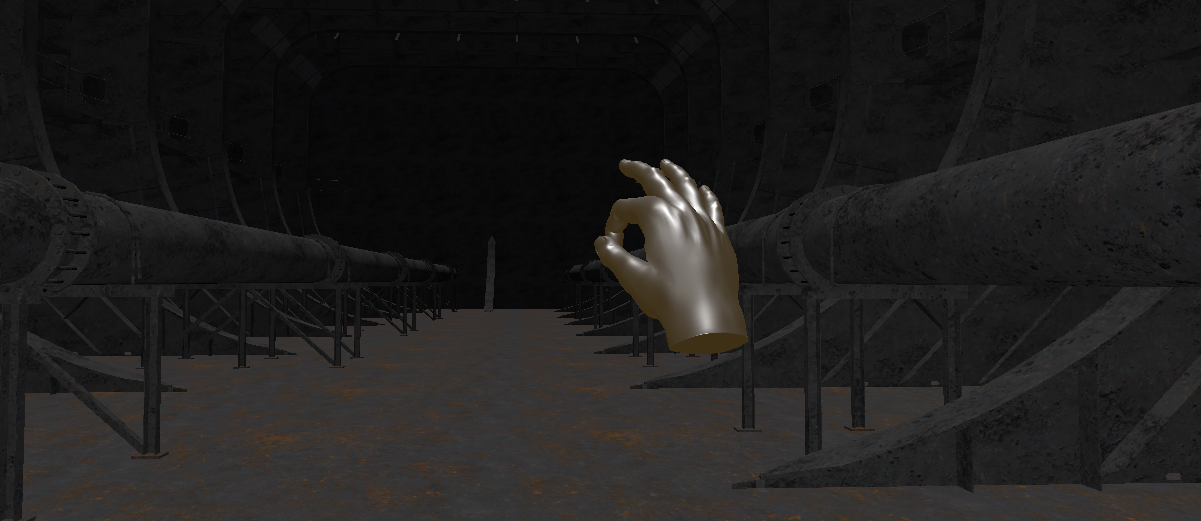
\includegraphics[width=\linewidth]{pictures/screenshots/gestures/pinch_detector2.png}
	\caption[The pinch gesture]{When the PinchDetector is active, i.e a pinch gesture is recognized, the hand is colored in a pale gold color.}
	\label{fig:pinch_detector2}
\end{figure} 

The \texttt{PinchDetectorStrict} and \texttt{PinchDetectorSlack} were originally one detector called \texttt{PinchDetector}, but was split up to represent two 
different options for the user. Both detectors utilize the base \textit{PinchDetector} script provided by the Leap Motion detection utilities, while the strict version
also uses the \textit{ExtendedFingerDetector}. The \texttt{PinchDetector} measures the distance between the tip of the thumb and index finger, and if these are below
a certain threshold (i.e the activate distance) the detector is active and signals \texttt{gestureCode}. If the distance grow larger than a set deactivate distance
the detector is deactivated. The activate distance used is 0.03 meter, while the deactivate distance is 0.06 meter. 

One problem with only having distance between the two finger tips as a criterion for the pinch gesture is that there would sometimes be false positives 
(i.e unintentional pinch gestures could occur). This was especially the case when attemping to perform the fist gesture as the distance between the tip of the
thumb and index finger is relatively small when the hand is a fist, and the application could thus sometimes perform a pinch gesture instead of a fist gesture.
Because of this the stricter version \texttt{PinchDetectorStrict} was created. This uses the same criterion as \texttt{PinchDetectorSlack}, but it also requires
that at least two fingers are extended. This is accompished by using the \textit{ExtendedFingerDetector} and \textit{DetectorLogicGate}. 
The finger states of the \textit{ExtendedFingerDetector} for all individual fingers are set to "either", meaning that, individually, each finger can 
be either extended or not extended, but on the "minimum extended" parameter 2 is set, while "maximum extended" is set to 5, 
meaning that anything between two and five fingers can be extended. 

\subsection{The PalmDownDetector}
\begin{figure}%[h!] %[H]
	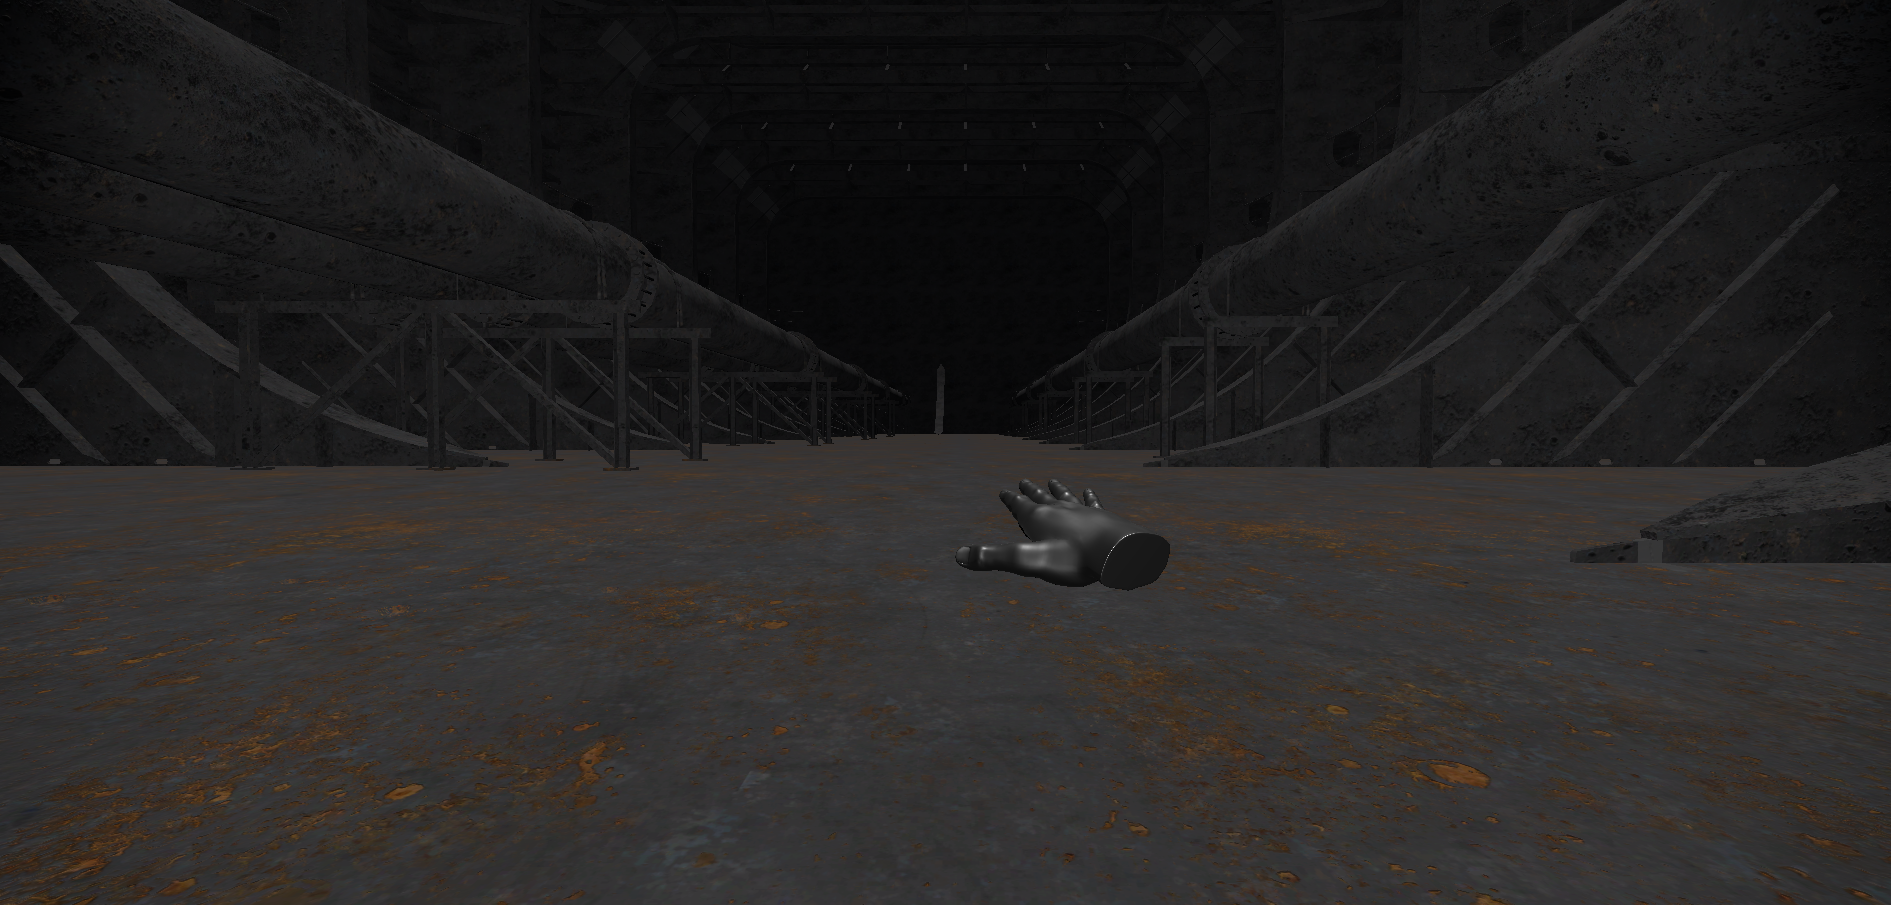
\includegraphics[width=\linewidth]{pictures/screenshots/gestures/palmdown_detector.png}
	\caption[The palmdown gesture]{When the PalmDownDetector is active, i.e a palm-down gesture is recognized, the hand is colored in a black.}
	\label{fig:palmdown_detector}
\end{figure}
The \texttt{PalmDownDetector} uses a PalmDirection detector and an ExtendedFinger detector, which is AND'ed by a DetectorLogicGate. 
The PalmDirectionDetector is configured to become active when the palm is pointing within 30 degrees of {0, -1, 0} (x = 0, y = -1, z = 0) direction, relative to the camera.
The coordinate system used functions just as if the three-dimensional axis had been drawn on the screen, so e.g.~ the coordinates {0, 0, 1} would be directly forward, while
{1, 0, 0} would be to the right.

The coordinates used for the PalmDirection Detector thus means that from the perspective of the camera, the palm should face directly downwords such that the 
palms are as parallell to the ground or table top.
The PalmDirectionDetector is also configured with an "On Angel" of 30 degrees and an "Off Angle" of 50. The detector is thus activated as long as the palm points within 
30 degrees of the desired direction, and is deactivated if the palm directions surpasses the threshold of 50 degree from the {0, -1, 0} direction.

The \texttt{PalmDownDetector} also used an ExtendedFingerdetector, as was covered in the previous section. This one is configured to require that 
the index-, middle, ring and pinky finger have to be extended, which the thumb can be either. 

\subsection{The PalmSideDetector}
\begin{figure}%[h!] %[H]
	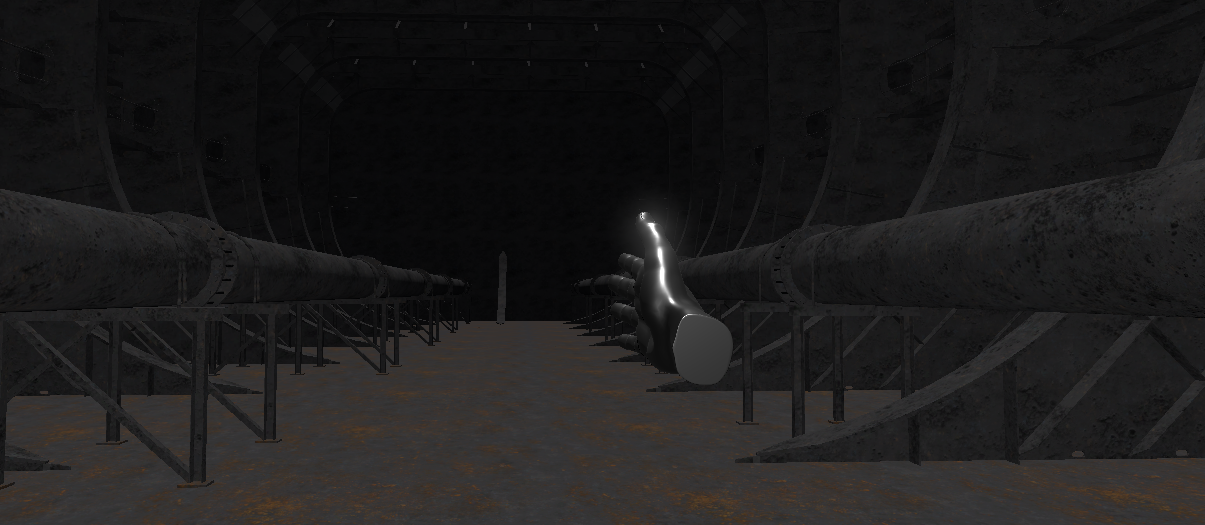
\includegraphics[width=\linewidth]{pictures/screenshots/gestures/palmside_detector.png}
	\caption[The palmside gesture]{When the PalmSideDetector is active, i.e a palm-side gesture is recognized, the hand is colored in a black.}
	\label{fig:palmside_detector}
\end{figure} 

The \texttt{PalmSideDetector} is quite similar to the \texttt{PalmDownDetector} and uses the same detectors, but with a different configuration. 
Although the settings used for the DetectorLogicGate and the ExtendedFingerDetector are very similar, the settings for the PalmDirectionDetector differs.
Unlike the \texttt{PalmDownDetector}, where both hands are required to point in the direction {0, -1, 0} to perform the gesture, the \texttt{PalmSideDetector} makes 
a distinction here. This is because requiring the palm direction {1, 0, 0} (right) is reasonable for the left hand, as it is within its natural range of motion, but
for the right hand this requires the whole arm to twist. The required palm direction for the left hand is thus {1, 0, 0} (right), and {-1, 0, 0} (left) for the right hand, both
with an "On Angel" of 30 degrees and an "Off Angle" of 50.

\subsection{The FistDetector}
\begin{figure}%[h!] %[H]
	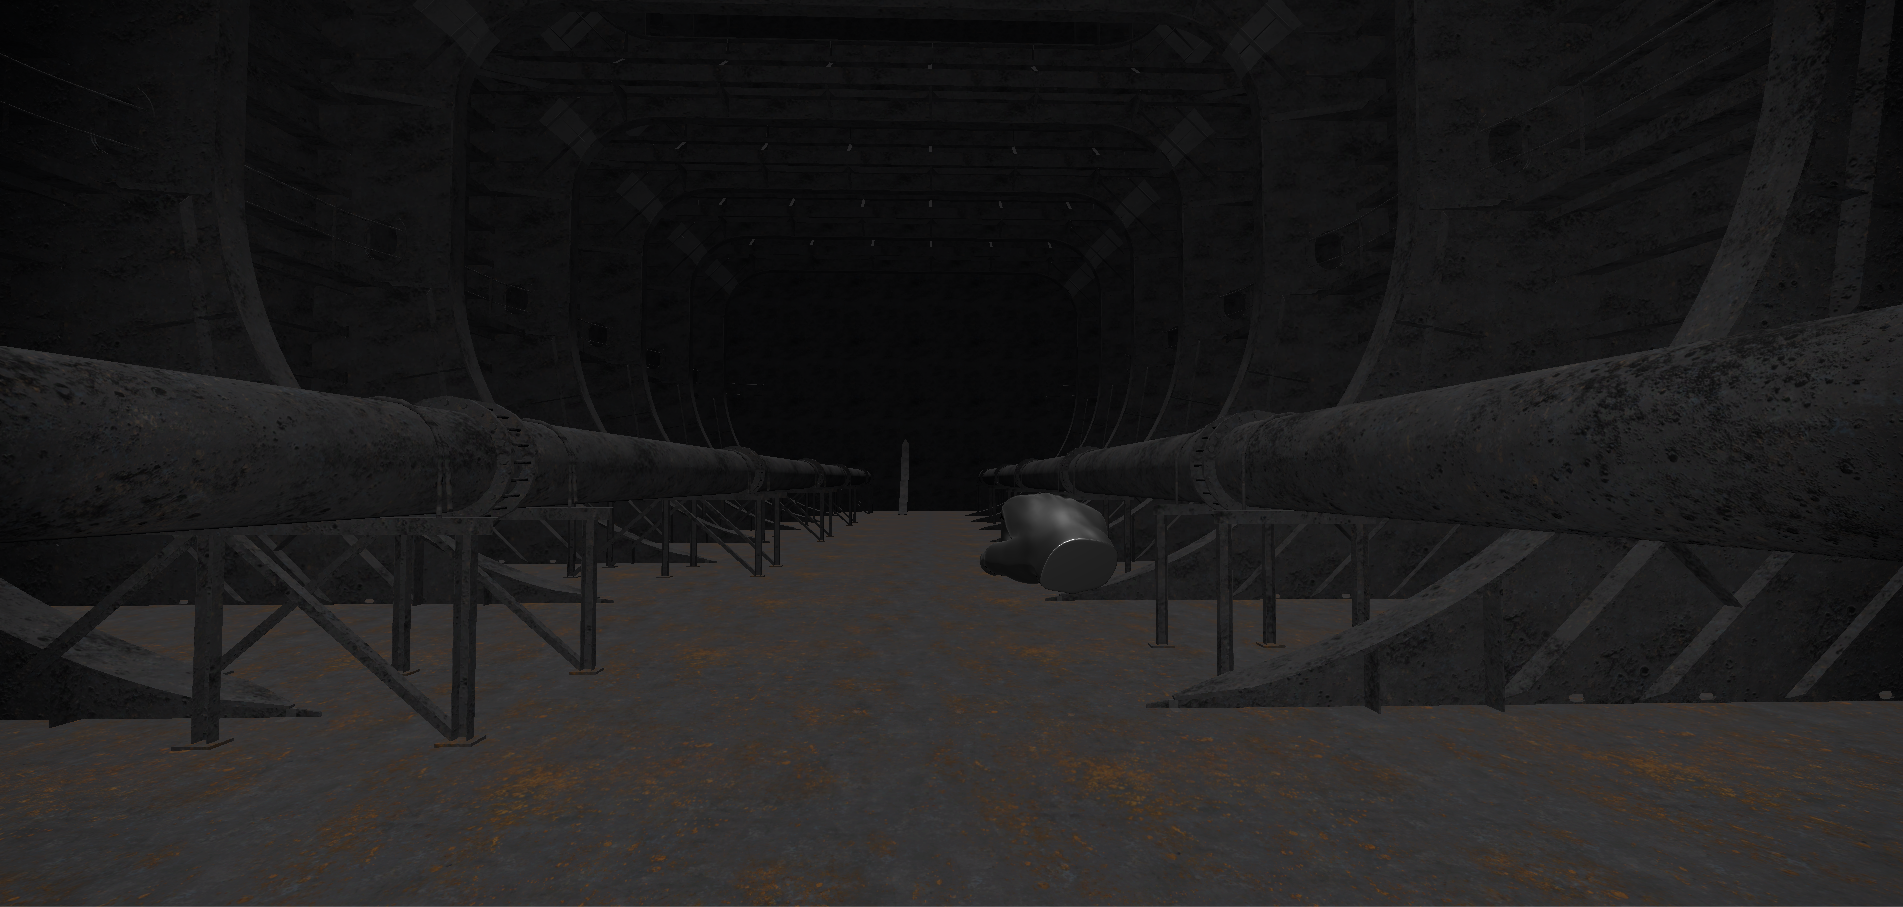
\includegraphics[width=\linewidth]{pictures/screenshots/gestures/fist_detector.png}
	\caption[The fist gesture]{When the FistDetector is active, i.e a fist gesture is recognized, the hand is colored in a black.}
	\label{fig:fist_detector}
\end{figure} 
The \texttt{FistDetector} is prehaps the simplest of the detectors and only uses the ExtendedFingerDetector.
The ExtendedFingerDetector is simply configured to require that no finger is extended. 
As such the minimum- and maximum amount of fingers extended are both set to 0, and all finger have their required state set to "Not Extended"

\subsection{The SinglePointDetector}
\label{sec:singlepoint_detector}
\begin{figure}%[h!] %[H]
	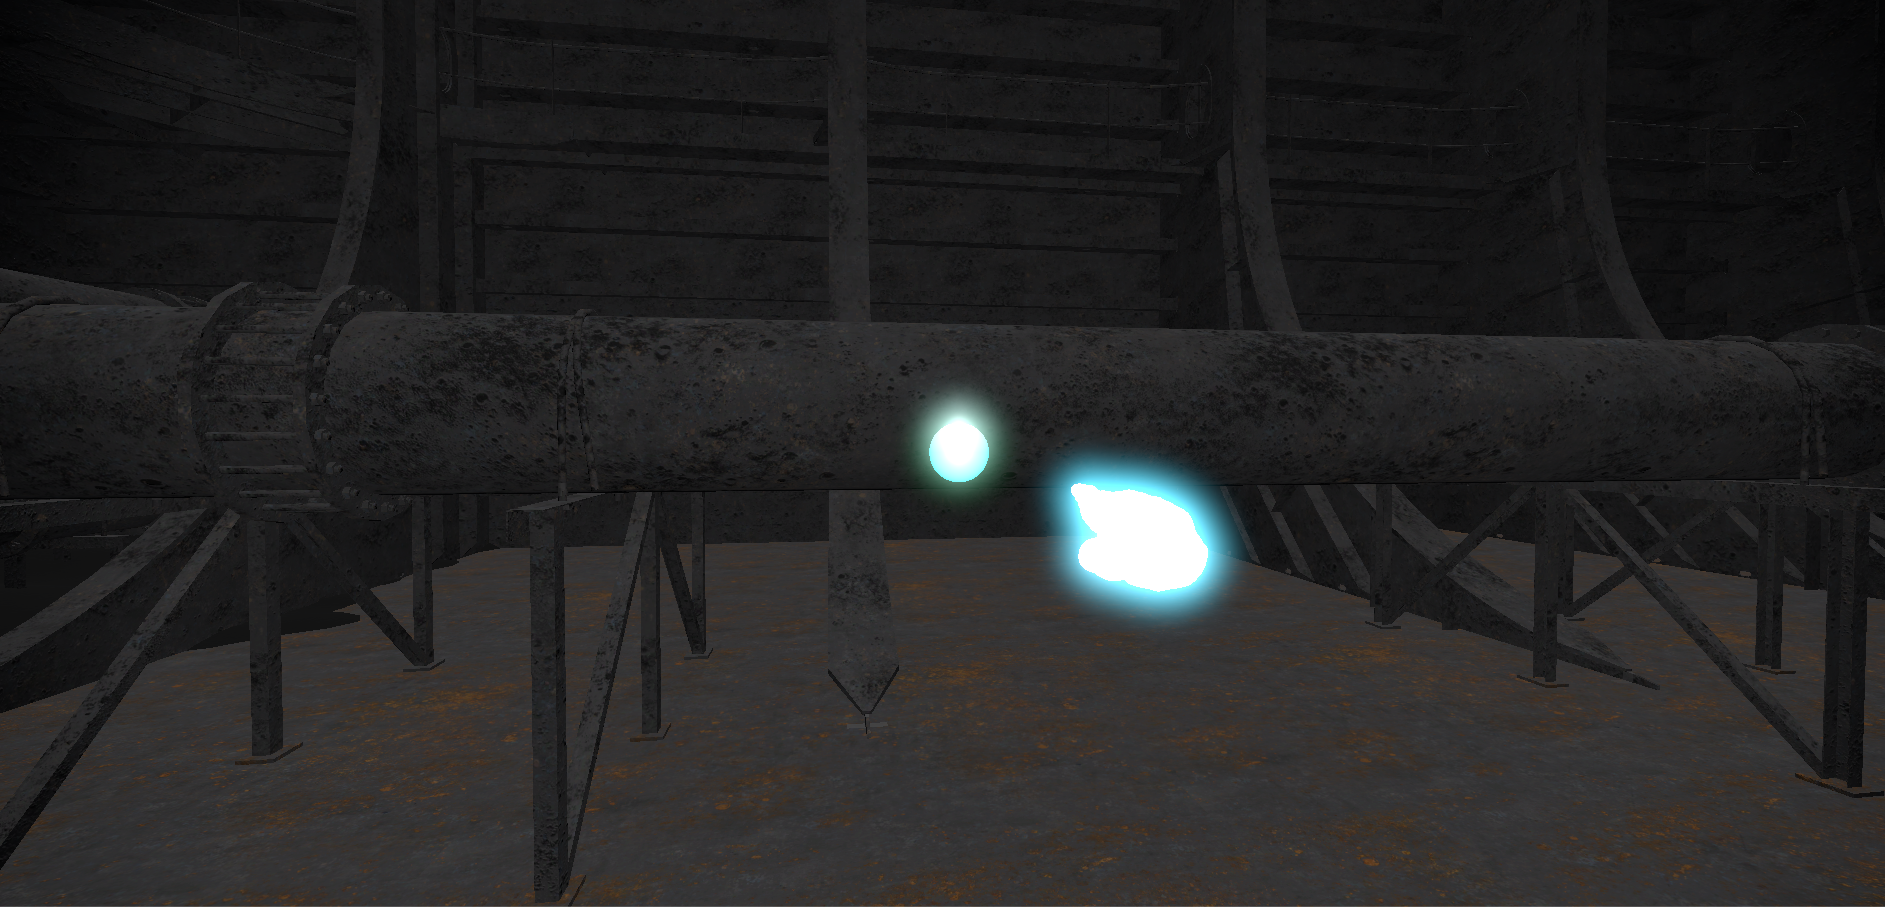
\includegraphics[width=\linewidth]{pictures/screenshots/gestures/singlepoint_detector.png}
	\caption[The single-point gesture]{When the SinglePointDetector is active, i.e a single-point gesture is recognized, the hand is colored in a glowing teal color.}
	\label{fig:singlepoint_detector}
\end{figure} 
The \texttt{SinglePointDetector} uses two detectors, ExtendedFingerDetector and FingerDirectionDetector, bound together with an AND-DetectorLogicGate.
The ExtendedFingerDetector here requires that the index finger is extended and that the middle-, ring- and pinky fingers are not extended (both thumb states are accepted).
The FingerDirectionDetector is set to be active when the index finger points within 15 degrees of the direction {0, 0, 1}, relative to the camera.
Both the "On Angle" and "Off Angle" settings are set to 15 in this detector, as, unlike the previously mentioned detectors, this one is not of a "continous nature".
Simply put, the previous gestures can last as long as the gesture is held, and while this is the case the application continously watches the active hands and responds to
hand movements. The single- and double point detectors are techniqually also continous and can last as long as the user desires, 
but as soon as these gestures are activated their discrete action is performed. After this action has been performed no other action will be performed by the same
and while the same gesture is kept. In the case of both the single- and double point detectors, an annotation is either placed or edited upon activation. 
If a user thus with to place an annotation and immediatly edit it, he or she has to use the approprate gesture, release the gesture and do the same gesture again.

\subsection{The DoublePointDetector}
\begin{figure}%[h!] %[H]
	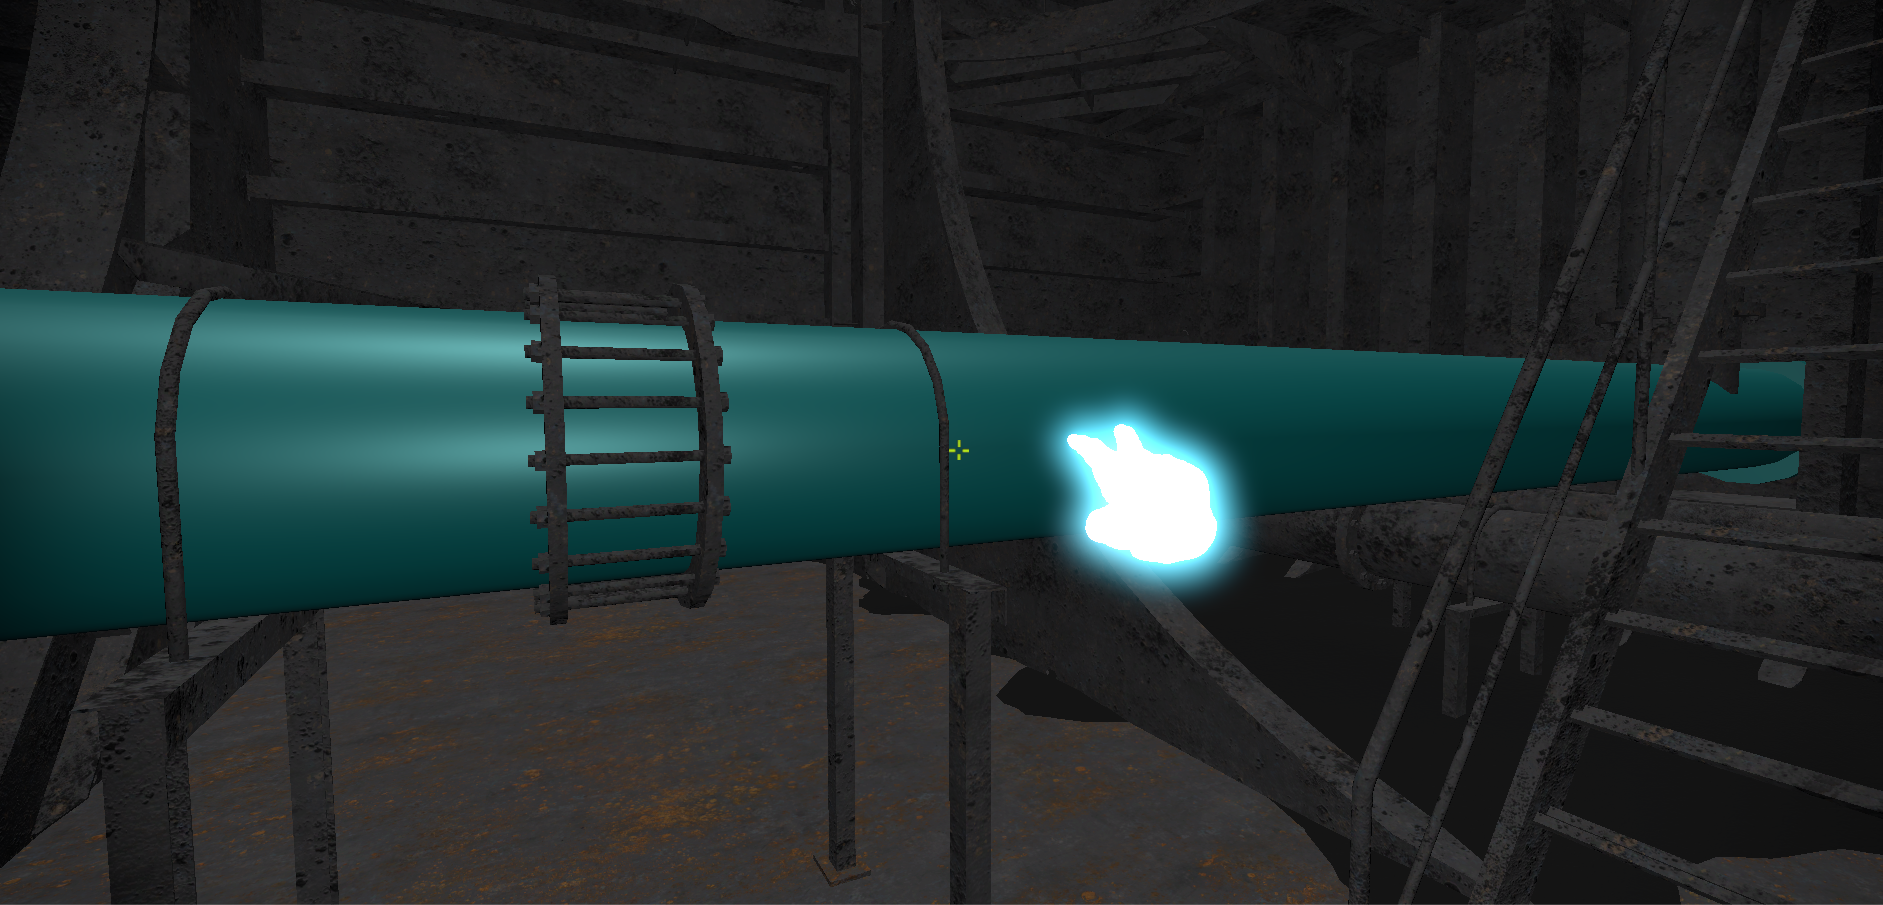
\includegraphics[width=\linewidth]{pictures/screenshots/gestures/doublepoint_detector.png}
	\caption[The double-point gesture]{When the DoublePointDetector is active, i.e a double-point gesture is recognized, the hand is colored in a glowing teal color.}
	\label{fig:doublepoint_detector}
\end{figure} 
The \texttt{DoublePointDetector} is similar to the \texttt{SinglePointDetector} and uses the same base detectors. 
The only implementational difference between this two is that the ExtendedFingerDetector is configured to require that both the index- and middle finger are extended, while
the ring- and pinky finger are contracted (both thumb states are accepted).